% Drawing 154/05-3 -- folder 154, batch 05, archive page 91 (PDF page 92).
% Transcription: dessin en couleur au milieu du bas de page : deux paires de droites rouges qui se croisent de part et d'autre d'une droite horizontale jaune-vert ($D$), prolongée en pointillé ; les points marqués $u$, $s$, $s'$, $v$ sur $D$ et $\alpha$, $\beta$ sur les droites rouges
% Kind: two pairs of crossing lines on a line D. Method 2 (schematic redraw from the facsimile). Status: ok.
% Notes: Middle of the foot of the left column: two pairs of red lines crossing, one just above, one just below the yellow-green line D, which is prolonged in dots at both ends; the points u, s, s', v on D and alpha, beta on the red lines; black marks at the crossings. D is not labelled on the facsimile.
% Coordinates: 1 unit = 1 mm = 1/100 of the crop width (bbox in page fractions: [0.193, 0.384, 0.329, 0.428]).
% Redrawn by Claude (claude-opus-5-5), issue #73, 2026-11-07; not checked by a human; not compiled (no TeX in the session).
% Rights: reproduces part of the work -- behind RENDER_TRANSCRIPTS, never published by itself.
\documentclass[tikz,border=3pt]{standalone}
\usepackage{amsmath,amssymb}
\usetikzlibrary{patterns,arrows.meta}
\tikzset{Or/.style={orange!90!black}, Ye/.style={yellow!80!orange}, Lg/.style={green!60!black!70}, Dg/.style={green!45!black}, Br/.style={brown!80!black}, Rd/.style={red!85!black}, Bl/.style={blue!70!black}, Gy/.style={black!40}, pencil/.style={black!45}, struck/.style={black!35}, mark/.style={circle,draw,inner sep=1.3pt}, pt/.style={circle,fill,inner sep=0.9pt}, opt/.style={circle,draw,fill=white,inner sep=1.1pt}}
\begin{document}
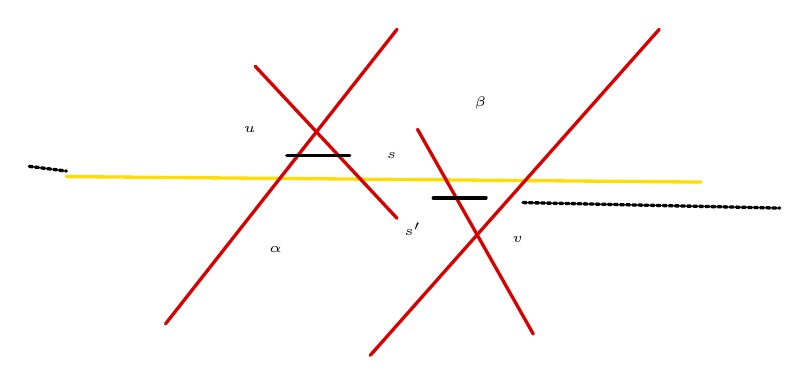
\begin{tikzpicture}[x=1mm,y=1mm,line cap=round,line join=round,font=\scriptsize]
\draw[Ye,very thick] (6.7,-22) -- (87.3,-22.7);
\draw[densely dotted,very thick] (2,-20.7) -- (6.7,-21.3);
\draw[densely dotted,very thick] (64.7,-25.3) -- (97.3,-26);
\draw[Rd,very thick] (30.7,-8) -- (48.7,-27.3);
\draw[Rd,very thick] (48.7,-3.3) -- (19.3,-40.7);
\draw[Rd,very thick] (82,-3.3) -- (45.3,-44.7);
\draw[Rd,very thick] (51.3,-16) -- (66,-42);
\draw[very thick] (34.7,-19.3) -- (42.7,-19.3);
\draw[very thick] (53.3,-24.7) -- (60,-24.7);
\node[inner sep=1pt] at (30,-16) {\tiny $u$};
\node[inner sep=1pt] at (48,-19.3) {\tiny $s$};
\node[inner sep=1pt] at (50.7,-28.7) {\tiny $s'$};
\node[inner sep=1pt] at (64,-30) {\tiny $v$};
\node[inner sep=1pt] at (33.3,-31.3) {\tiny $\alpha$};
\node[inner sep=1pt] at (59.3,-12.7) {\tiny $\beta$};
\end{tikzpicture}
\end{document}
